% ---
% Capítulo 2
% ---
\chapter{Fundamentos Teóricos}
\label{chap:conceitos}

\todo[inline]{\textbf{NOTA}: Referencial ou embasamento teórico - texto no qual se deve apresentar os aspectos teóricos, isto é, os conceitos utilizados e a definição dos mesmos. \textbf{AQUI VOCÊ DEVE APRESENTAR UM TEXTO PARA INTRODUZIR OS CONCEITOS QUE SERÃO ABORDADOS.}}

\section{Divisão a ser definida com o aluno de acordo com o tema}

\todo[inline]{\textbf{NOTA}: A ideia de cada seção é abordar um aspecto téorico, contendo a definição, um exemplo e como este conceito se relaciona no seu trabalho. Segue \textbf{um exemplo} de apresentação de código na linguagem de programação C que pode ser utilizado na apresentação de conceitos.}

\begin{figure}[thp]
	\caption{\label{fig:program_test} Exemplo de código}
    \centering
    \begin{subfigure}{0.4\textwidth}
    \centering
    \begin{lstlisting}[language=C]       
double custo(double entrada)
{
  if (entrada < 0) 
  {
    return -1;
  }
  if ((entrada * 1.5) <= 0)) 
  {
    return -1;
  }
  if(entrada > 50) 
  {
    return 1.25*entrada;
  }
  return 1.5*entrada;
}
	\end{lstlisting}
    \caption{Código C}
  \end{subfigure}%    
  \begin{subfigure}{.05\textwidth}
    \hfill
  \end{subfigure}%    
  \begin{subfigure}{.4\textwidth}
    \centering
\begin{lstlisting}[language=C]   
TEST_CASE_1()
{
  double result;
  result = custo(0.49)
  assert(result == 0.735);
}
TEST_CASE_2()
{
  double result;
  result = custo(51)
  assert(result == 63.75);
}
\end{lstlisting}
    \caption{Código de Teste}
  \end{subfigure}%
    \legend{Fonte: Própria do autor.}
\end{figure}

%%%%%%%%%%%%%%%%%%%%%%%%%%%%%%%
\subsection{Subdivisão de acordo com a necessidade de subdivisão}
\label{subsect:fig}

\todo[inline]{\textbf{NOTA}: Segue um exemplo de uso de figura}

A Figura~\ref{fig_grafico} apresenta o fluxo de microserviços.

\begin{figure}[h!]
    \caption{\label{fig_grafico}Fluxo de microserviços.}
	\begin{center}
	    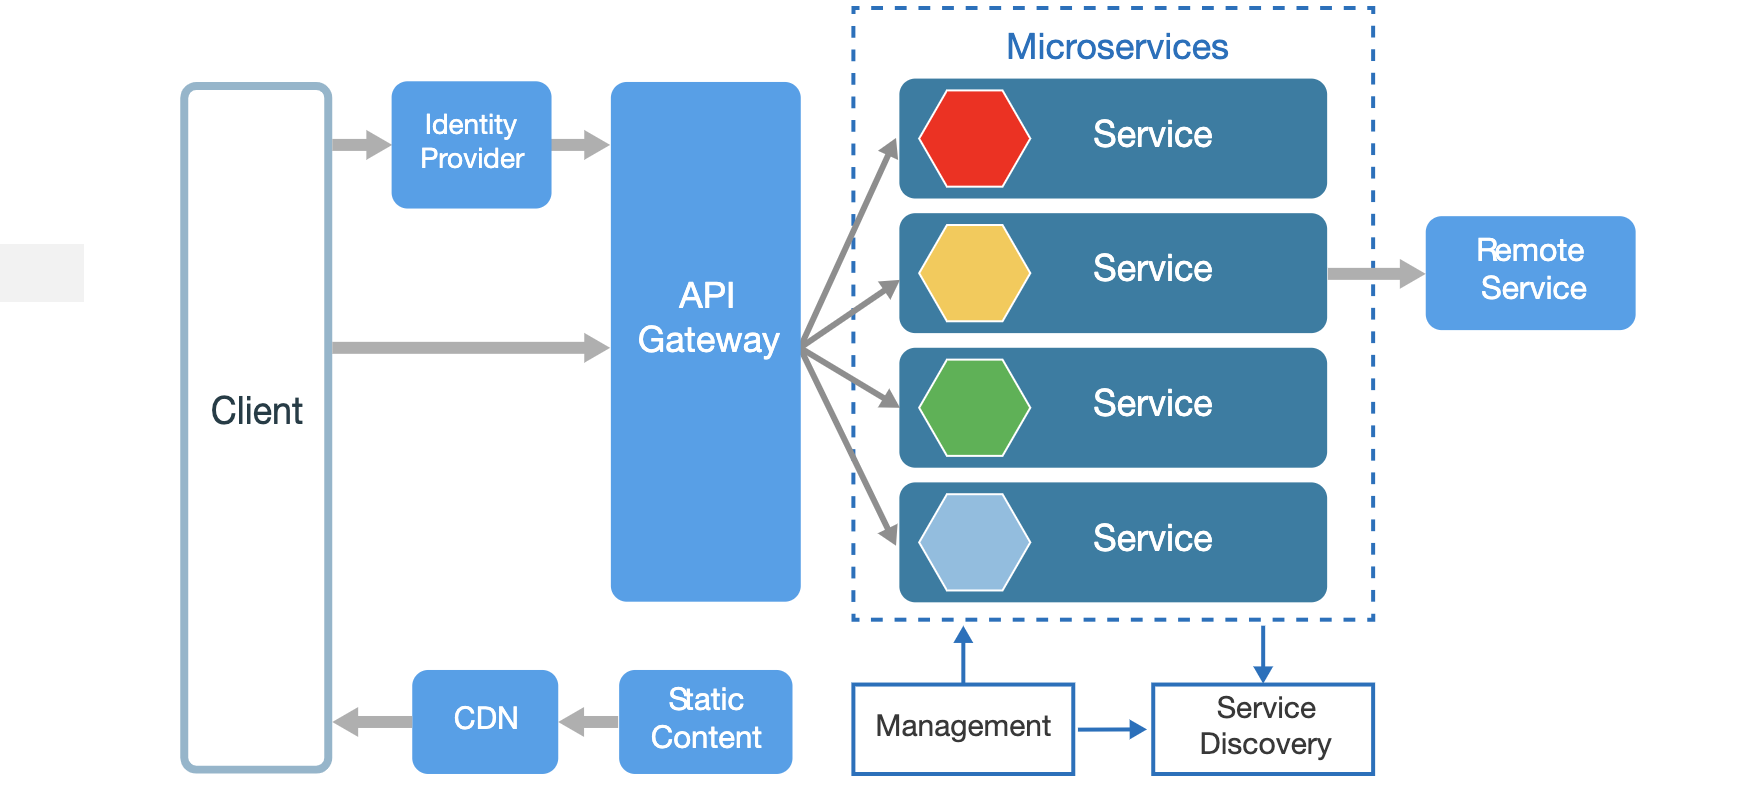
\includegraphics[scale=0.2]{images/arch.png}
	\end{center}
	\legend{Fonte: Internet em \cite{microservice:2019}.}
\end{figure}

\todo[inline]{\textbf{NOTA}: Continuação do texto. Segue um exemplo de apresentação de um algoritmo} 

O algoritmo na ~\autoref{fig:algoritmo_assert_free} visa a identificação da liberação de memória:

\begin{figure}[H]
	\caption{\label{fig:algoritmo_assert_free}Algoritmo para validar desalocação de endereço}
	\begin{center}
\begin{algorithmic}[1]
\Function{IsValidFree}{$addr, mallocLog$}
\State $i\gets tamanhoDoLog(mallocLog) - 1$
\While{$i\geq0$} \Comment O($m$)
\State $row\gets mallocLog[i]$
\State $i \gets i-1$
\If{$(row.addr = addr)$} \Comment O(1)
\If{$row.isFree$} \Comment O(1)
\State \textbf{return} FALSE
\Else
\State \textbf{return} TRUE
\EndIf
\EndIf
\EndWhile
\State \textbf{return} FALSE
\EndFunction
\end{algorithmic}
\end{center}
\legend{Fonte: Própria do autor}
\end{figure}


\section{Divisão a ser definida com o aluno de acordo com o tema}

\todo[inline]{\textbf{NOTA}: Segue um exemplo de uso de referência de seção e de equações.}

Referência a Seção~\ref{subsect:fig}. Um exemplo de exemplo de Equação~\ref{eq:poli}:

\begin{equation}
\label{eq:poli}
    f(n) = 4x^2 + 2y*12
\end{equation}

Outro exemplo de matemática em Latex: Calcule as raízes da equação $x^2 + 12x - 13 = 0$.
\begin{equation}
 x = \frac{-12 \pm \sqrt{12^2 - (4)(1)(-13)}}{(2)(1)} = \frac{-12 \pm \sqrt{196}}{2} = \frac{-12 \pm 14}{2} = -6 \pm 7
\end{equation}



\section{Destaques conceituais para pesquisa}

\todo[inline]{\textbf{NOTA}: Nesta seção deve-se apresentar uma relação/contextualização para cada conceito apresentado, ou seja, como os conceitos se integram e como serão utilizados no trabalho apresentado.}




	
	